\documentclass[../main/thesis_msc.tex]{subfiles}

\begin{document}

\chapter{Introduction}

\section{Low frequency astronomy}

\begin{tcolorbox}[titlerule=0.5mm,title=\textbf{{\Large History of radio astronomy}}]
$\begin{array}{ll} 
1933 & \textrm{At the Bell Labs, Karl Jansky was trying to figure out the source of interference at short wavelength}\\ 
     & \textrm{in the transatlantic wireless communication, and discovered radiation at 20.5~MHz frequency that}\\
     & \textrm{moved across our sky and figured out that it was not from earth.} \\
1937 & \textrm{Grote Weber speculated that these signals were thermal in nature and built a parabolic reflector}\\
     & \textrm{radio telescope with a diameter of 9.5~m and made the first radio map depicting the galactic plane}\\
     & \textrm{and parts of the sky at 160~MHz, and published the paper \citep{grote} in 1944.}\\
1940s & \textrm{Innovations during the Second World War in the RADAR technology further helped the research}\\
     & \textrm{J.S. Hey, England and G. C. Southworth discoved that sun was radiating radio emission. This}\\
     & \textrm{was followed by discovery of fluctuation in cosmic radiation at radio frequency by  J.S. Hey,}\\
     & \textrm{S.J. Parsons, and J.W. Phillips \citep{fluctuation}. Several discrete radio sources were also}\\
     & \textrm{identified. Radio emission from meteors was also studied.}\\
1950s & \textrm{In the papar \citep{h1}, H. I. Ewen and E. M. Purcell observed the H1 21~cm line from}\\
     & \textrm{galaxy, as predicted by van de Hulst in 1945. Several radio observatories came to life in this}\\
     & \textrm{such as Cambridge observatory that helped in producing the 2C and 3C catalogues, and was the}\\
     & \textrm{decade first to make use of aperture synthesis technique. Radio emission}\\
     & \textrm{from Jupyter was also studied at 22~MHz and 3~GHz  \citep{jupiter}.}\\
1960s & \textrm{A. Penzias and R. Wilson using the Holmdel Horn Antenna at the Bell Labs made one of the most}\\
     & \textrm{important astrophysical discoveries: the Cosmic Microwave Background, for which they were}\\
     & \textrm{awarded the Nobel prize in 1978. This decade also marked the discovery of pulsars by J. Bell}\\
     & \textrm{in her article "Little Green Men, White Dwarfs or Pulsars?" \citep{jocelyn} Sir M. Ryle}\\
     & \textrm{and A. Hewish received the Nobel prize in 1974 for this discovery.}\\
1970s & \textrm{Hulse and Taylor discovered the first binary pulsar system at Arecibo, and thus proved the}\\
     & \textrm{presence of Gravitational wave radiation, after conducting pulsar timing for nearly 20 years}\\
     & \textrm{\citep{binary}. They were awarded the Nobel prize for this discovery in 1993.}\\
     & \textrm{The first global radio telescope was formed, in 1976 to observe water maser sources.}\\
1980s & \textrm{The need to better resolution gave rise to construction of interferometers such as TPT}\\
     & \textrm{ in Clark Lake observing at the frequency of 57.5~MHz. The first self calibration for VLA}\\
     &\textrm{images was done. Astronomical Image Processing Software (AIPS) was released. }\\
1990s & \textrm{VLA system obsering at 74~MHz frequency was used. Planck black-body spectrum for the CMB}\\
     & \textrm{was measured, and the anisotropy was discovered for the first time using COBE satellite.}\\
     & \textrm{\citep{cobe}. Mather and G. Smoot were awarded Nobel prize for this discovery in 2006.}
\end{array}$
\end{tcolorbox}
Due to the need for higher resolutions, studies were mostly focussed on higher frequencies\footnote{Angular resolution of a single dish telescope can be written as $\theta = \alpha\frac{\lambda}{d}$~rad, where `$\lambda$' is the wavelength of observation and `d' is the diameter of the telescope (both in terms of meters). In case of an interferometer, the resolution is written as $\theta = \alpha\times \frac{\lambda}{D}$~rad, where D is the distance between the telescopes (in meters). Here $\alpha$ depends on the array configuration and the weighing scheme used during imaging \ref{sec:weighting}. In reality, it also depends on the array configuration and the declination of the source. For LOFAR, the resolution varies between 0.5$\deg$ to sub-arcsecs.} during 1970 to 2000. Several higher frequency telescopes were made- VLA, ATCA, GMRT, MERLIN and single dish telescopes such as Effelsberg, Arecibo and Lovell. Interest in low frequency radio astronomy begin when many sources were seen to have inverted spectra due to synchrotron self-absorption or free-free absorption\footnote{We will visit these phenomena in section \ref{invt.spec}.}. NRAO and the Naval Research Laboratory completed the implimentation of a VLA at 73.8~MHz in 1998 and found that ionospheric phase shifts posed the biggest difficulty in calibrating data. It was found that self-calibration could help with this \citep{74MHz}. In the paper \citep{vlss}, 70,000 sources were catalogues including several extra-galactic and galactic sources such as high redshift galaxies, galaxy clusters, pulsars and Supernove Remenants (SNRs) at 77~MHz. It covers almost  95\% of the 3$\pi$~sr of sky above -30~deg declination. This survey is very useful for calibration in LOFAR. This survery has been revised to give 95,000 sources in \citep{vlss2}. In the paper \citep{ska}, a 1~km$^2$ array was proposed so as to study the neutral hydrogen at cosmological distances, called the Square Kilometer Array (SKA). Due to cost constraints, the concept of Phased Arrays \citep{lof1} using dipole antennae was proposed, which then gave rise to LOFAR.

\subsection{LOw Frequency array- LOFAR}    
LOFAR or LOw Frequency Array is a radio interferometer mainly located in the Netherlands. It consists of two types of receiving elements: the Low Band Antennae (LBA) that covers the frequency range of 10-90~MHz, and the High Band Antennae (HBA) that covers the frequency range from 110-250~MHz. It is interesting to note that the pointing in LOFAR is done by applying digital delays to elements of individual stations. The LBA (shown in Fig. \ref{lba}) in reality can only operate between the frequncy range of 30-80~MHz due to the presence of Radio Frequency Interference(RFI) at the lower frequency regime and the commercial FM band at the higer regime. An LBA dipole can detect two orthogonal linear polarisations, with an all-sky sensitivity. The diploles themselves do the make up the elements to do beamforming. The HBA (shown in Fig. \ref{hba}) can reach frequency only upto 240~MHz due to RFI. 16 antennae are grouped under one ``tile", and each of these tiles can form a ``tile beam". Each tile does the beamforming with the help of an analogue beamformer that adds a delay to each dipole.

\begin{figure}[h]%
    \centering
    \subfloat[]{{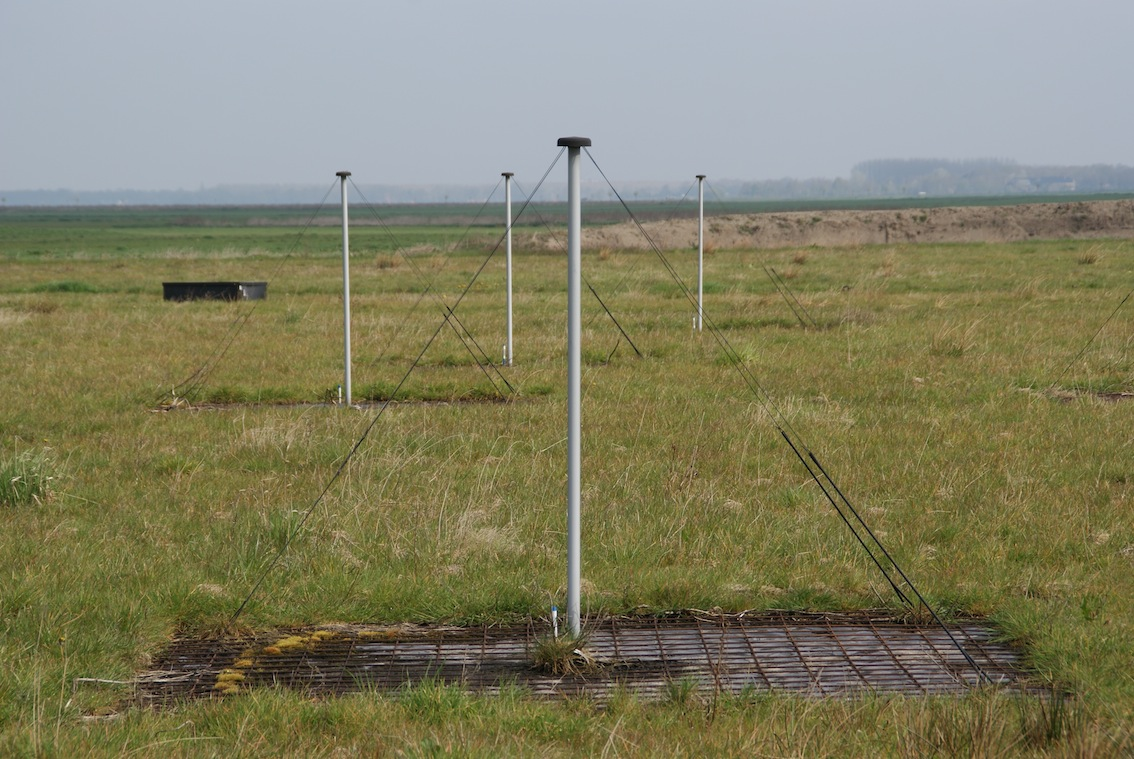
\includegraphics[width=5cm]{lba.png} }%
    \label{lba}}
    \qquad
    \subfloat[]{{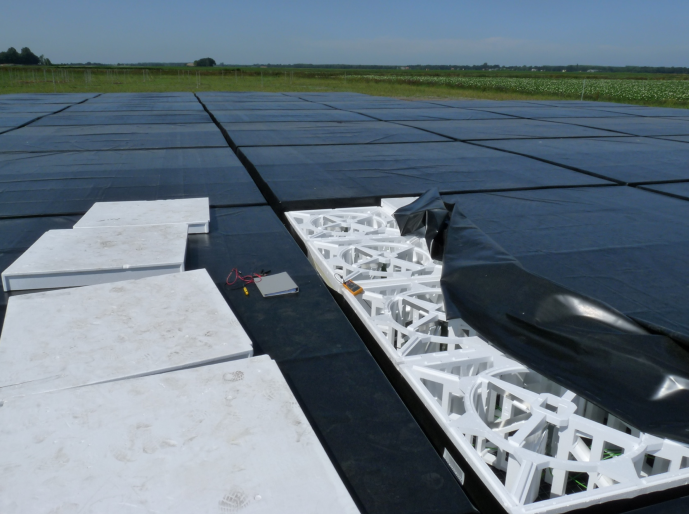
\includegraphics[width=4.5cm]{hba.png} }
    \label{hba}}%
    \caption{The different Antenna types in LOFAR. \textit{Left:} Low Band Antenna is held upright by the two copper wires connected to its top that help in detection of the two polarisations, and the ground mesh \citep{lba}. \textit{Right:} Each High Band Antenna tile has 16 aluminium elements held together by an expanded polystyrene structure \citep{LOFAR}}%
\end{figure}

It has a dense core i.e., it has numerous short baselines that are very helpful in the study of diffuse emission. LOFAR currently has 24 core stations (CSs) located in Exloo, Netherlands, and 14 remote stations (RSs) located all over the Netherlands. These stations have 96 LBAs and 48 HBAs with 48 digital Receiver Units (RCUs). These arragements can be seen the Fig. \ref{lofar_arrangement}. The international stations (ISs) are present in Germany (5 stations), Great Britain (1 station), France (1 station) and Sweden (1 station). A summary of the arrangement and other properties of LOFAR are given in Table \ref{lofar_specs}. 

\begin{table}[t]
        \centering
        \begin{tabular}{ccc}
            \toprule
            \textbf{Characteristic} & \textbf{Value} & \textbf{Comments} \\ \midrule
            Frequency range & 10-90~MHz & LBA \\
              				& 110-190~MHz & HBA \\ \\
            Shortest baseline & 68m & among CSs, RSs and ISs (unprojected values) \\ \\
            Maximum baseline & 3.5~km & CSs \\
            				 & 121~km & RSs \\
            				 & 1158~km & ISs \\ \\
            Number of Polarisations & 2 & \\ \\
            Bandwidth & 48~MHz & 16-bit mode \\
              		  & 96~MHz & 8-bit mode \\ \\
            Maximum number of & 244 & 16-bit mode\\
            simultaneous beams & 488 & 8-bit mode\\
            \bottomrule
        \end{tabular}
        \caption{LOFAR specifications, all obtained from \citep{LOFAR}}
        \label{lofar_specs}
    \end{table}
    

\begin{figure}[h]
	%\centering
	\subfloat[]{{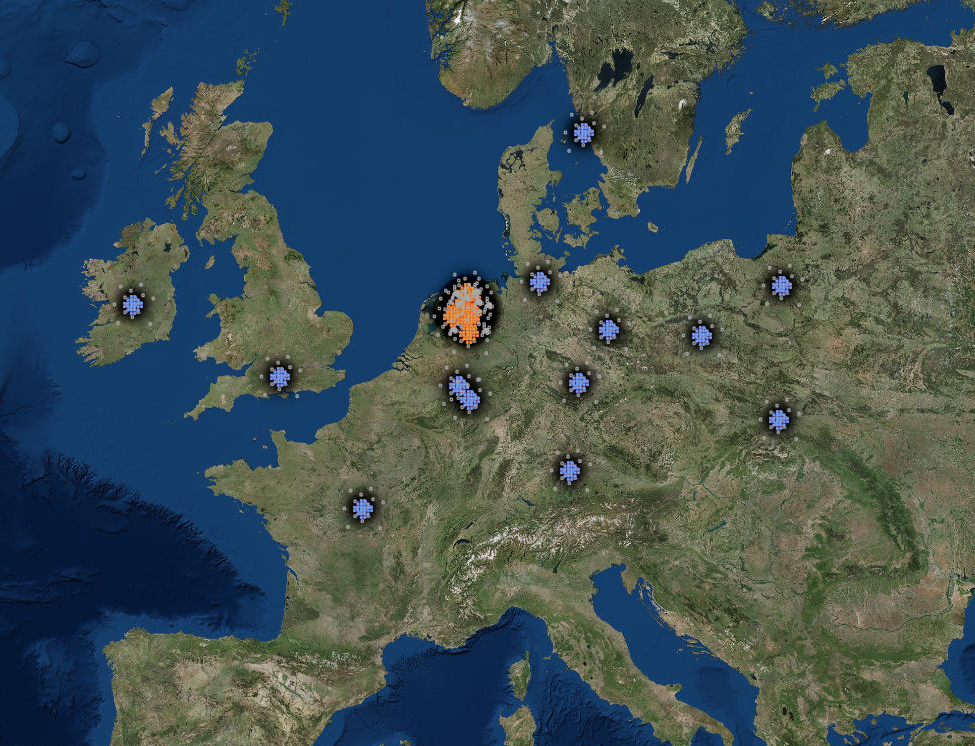
\includegraphics[width=5cm, height=4cm]{lofar_arrangement.png}}}
	\centering
	\subfloat[]{{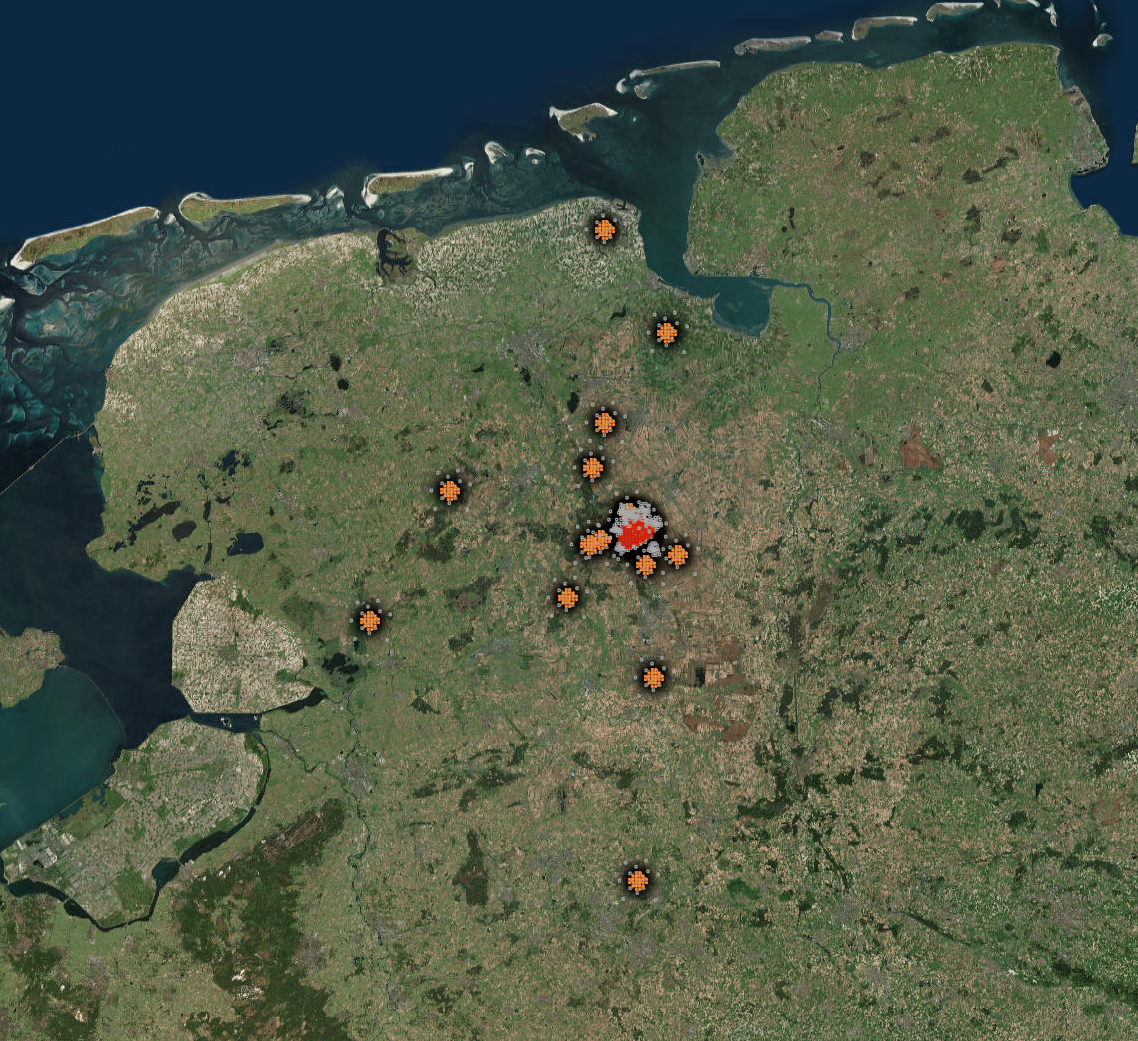
\includegraphics[width=5cm, height=4cm]{lofar_arrangement_core.png}}}
	\caption{Arrangement of the LOFAR stations in Europe. \textit{Left:} The blue regions represent the international stations. The orange regions in the represent the remote stations. \textit{Right:} On a closer look, the red regions represent the core stations. These images were obtained from \url{http://astron.nl/lofartools/lofarmap.html}}
	\label{lofar_arrangement}
	\end{figure}

The data from both LBA and HBAs are sent to the receiver unit (RCU), where digitisation happens through coaxial cables. Then the beam-forming is done int he digital electronics section. After that, the signal is either sent to the Cobalt correlator in Groningen or recorded and delt with locally based on the observing mode. LOFAR has three main observing modes that are explained in the Table \ref{moooo}. 


\begin{table}[h]
\centering
\begin{tabular}{cc}
\toprule
\textbf{Modes} & \textbf{Description}\\ 
\midrule
Interferometric & Gives visibility data to be used in surveys and for single souce imaging. \\
Beam Formed & This is used when high time resolution is needed e.g., for pulsars, cosmic rays, etc. \\
Direct Storage & Uncorrelated data is recorded locally for single sdtation all sky imaging\\ & or local Trasient Buffer Board (TBB) experiments.\\
\bottomrule
\end{tabular}
\caption{The LOFAR imaging modes}
\label{moooo}
\end{table}

The data streams from the individual dipole antennae are sent to the Central Processing (CEP) facility located in Groningen through a dedicated network high speed fibres. The data is then processed in the Blue Gene/P supercomputer. During this processing, the signal from the stations is correlated, and the beam-forming is done. After this, the data is given to the storage cluster. The data is processed using several reduction pipelines before being stored in the LOFAR long term archive (LTA) for scientific purposes. 
The CEP4 cluster, part of the LOFAR clusters, is used to do the initial processing and calibration using pipelines on the data from the Cobalt correlator (in Groningen). Another cluster- CEP3, used by LOFAR users to decide the strategy to be used for calibration. Once the data has been processed, it is made available on Long Term Archive (LTA).\\

\noindent Some of the packages used for the calibration of LOFAR data are: Astronomical Image Processing Software(AIPS) \citep{aips}, Common Astronomy Software Applications (CASA) \citep{casa}, AOFlagger (helps in flagging RFI) \citep{aoflagger}, SAGECal (calibration package), dysco (compressing storage manager for measurement sets) and several others, which will be visited upon during the course of the thesis.


Some of the performance metrics of LOFAR are described below:
\begin{itemize}
\item The rate of change of the ionospheric phase above Netherlands is 1rad per 15s in the 110 to 190~MHz band \citep{LOFAR}. For LBA, water may affect the gain by the order of 10\%,  though HBA amplitudes remain pretty stable. These effects of inonosperic phase shift can be significantly depreciated using the method of self- calibration \ref{self-cal}. 
\item The angular resolution of the observation depends on the declination of the source, and the array configuration. For LOFAR, it is from 0.5~$\deg$  to sub-arcsec levels. 
\item One one the factors that affects the image quality id the uv coverage. As can be seen from the Fig.\ref{uv}, we can easily see that LOFAR has a very dense core and there are several long baselines, for better resolution.

\begin{figure}[h]
\centering
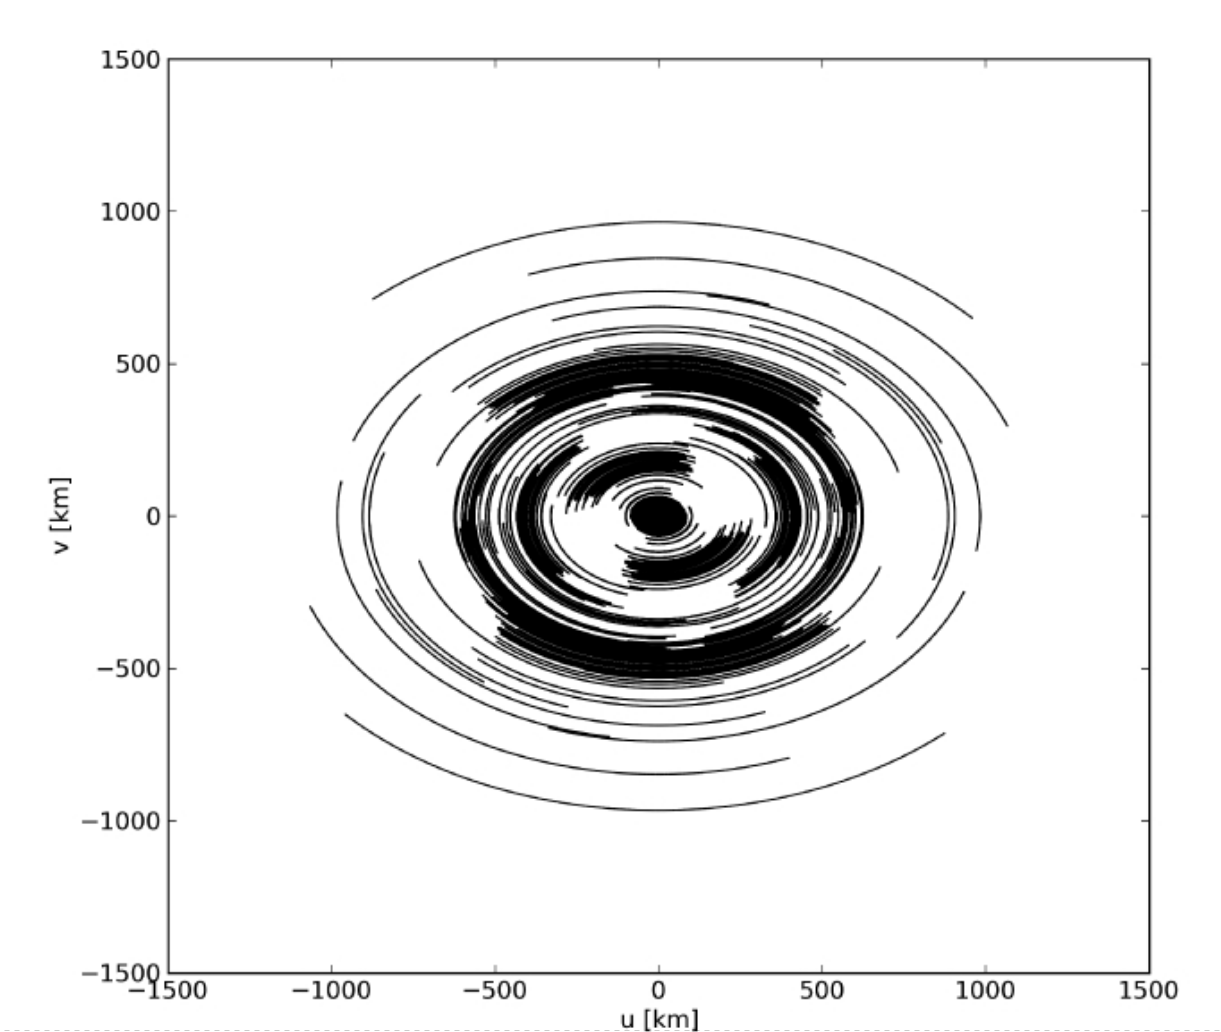
\includegraphics[scale = 0.2]{uvcoverage.png}
\caption{The uv coverage of LOFAR including all core, remote and international stations \citep{LOFAR}. The simulation of this uvcoverage is based on a hypothetical 6 hour observation of a source at a declination of 48~$\deg$ between 30-78~MHz using single beam with bandwidth of 48~MHZ}
\label{uv}
\end{figure}

\item The bandpass of LOFAR is affected by several factors: the station beam- which is in itself frequency dependant, the interaction between the antenna elements and the low noise amplifier (LNA). Inorder to take care of this, a digital correction is applied withon each 0.2~MHz subband.
\item The Field of View of LOFAR ranges from 2 to 1200~$\deg ^2$, and is given by:
\begin{equation}
\textrm{FoV}=\pi\left(\frac{FWHM}{2}\right)^2
\end{equation}

\end{itemize}


\subsection{Radio Interferometry Measurement Equation- RIME formalism}
\label{sec:rime}

The calibration techniques used for LOFAR are based on RIME formalism, which is explained in the section \ref{sec:rime}. The explaination closely follows the one given in \citep{rime}, since the Direction Dependant Effects (DDE) are well explained in it. This section describes the calculation of RIME from the voltages obtained at the antennae.\\

\noindent Consider a quasi-monochromatic source giving out a signal. This can be represented by a complex vector \textbf{\textit{e}} (the ``original signal"), and be written in the form of a matrix using an orthogonal coordinate system \textit{xyz}, with `\textit{z}' along the direction of propagation.

\begin{center}
\(
\textbf{\textit{e}} = 
  \begin{pmatrix}
    e_x \\
    e_y
  \end{pmatrix}
\)
\end{center}

\noindent The signal encounters multiple effects on its path towards the antennae. These effects are assumed to affect the signal \textit{\textbf{linearly}}. The signal changes to \textbf{\textit{e$^\backprime$}} due to these effects and can be written in the form given in the equation \ref{eq}.

\begin{equation}
\textbf{\textit{e$^{\backprime}$}} = \underbrace{\textbf{\textit{J}}_n \textbf{\textit{J}}_{n-1} ..... \textbf{\textit{J}}_1}_{\textbf{Jones chains}} \textbf{\textit{e}} = \textbf{\textit{J}} \textbf{\textit{e}} 
\label{eq}
\end{equation}

\noindent Here, \textit{\textbf{J}} is a 2$\times$2 complex matrix known as Jones matrix. Since there are multiple efects along the path of the signal, the Jones chain is written taking all these effects into account and the final cumilative Jones matrix can be written as \textit{\textbf{J}}.

\noindent If a and b are two linear dipole feeds, the signal one reaching and gets converted to complex voltages $v_a$ and $v_b$ representing the two polarisations. 

\begin{equation}
\textrm{
\(
\textbf{\textit{v}} = 
  \begin{pmatrix}
    v_a \\
    v_b
  \end{pmatrix}
\ = \textbf{\textit{J}} \textbf{\textit{e}} \)
}
\label{J}
\end{equation}

\noindent An interferometer consists of several antennae elements, so let us consider two such spacially separated elements - \textit{p} and \textit{q}, giving independant voltage vectors $\emph{v}_p$ and $\emph{v}_q$.  Their voltages are correlated to give the visibility matrix V$_{pq}$. Hence, the visibility matrix can be written as:

\begin{center}
\(
\textrm{V}_{pq} = 2
  \begin{pmatrix}
    \langle v_{pa}v^*_{qa} \rangle & \langle v_{pa}v^*_{qb} \rangle \\
    \langle v_{pb}v^*_{qa} \rangle & \langle v_{pb}v^*_{qb} \rangle
  \end{pmatrix}
\)
\end{center}

\noindent Here, $v^*$ represents the complex conjugate of $v$. V$_{pq}$ can be written as matrix product of $\emph{v}_p$ and complex conjugate of $\emph{v}_q$. \textit{H} represents the conjugate transpose operation.
\begin{equation}
\textrm{V}_{pq} = 2\langle v_{p}v^H_{q} \rangle
\label{H}
\end{equation}
 
\noindent Combining equations \ref{J} and \ref{H}, we get:
\begin{equation}
\textrm{V}_{pq} = 2\langle \textbf{\textit{J}}_{p}(\textbf{\textit{ee}}^H) \textbf{\textit{J}}_{q} \rangle
\end{equation}

\noindent We assume that \textbf{\textit{J}}$_{p}$ and \textbf{\textit{J}}$_{q}$  are constant over the averaging interval.

\begin{equation}
\textrm{V}_{pq} = 2\langle v_{p}v^H_{q} \rangle = 2\textbf{\textit{J}}_p \begin{pmatrix}
    \langle e_{x}e^*_{x} \rangle & \langle x_{x}e^*_{y} \rangle \\
    \langle e_{y}e^*_{x} \rangle & \langle e_{y}e^*_{y} \rangle
  \end{pmatrix} \textbf{\textit{J}}^H_q 
\end{equation}
\noindent A relation can be obtained between the source signal and Stokes parameters (I, Q, U, V) as shown in \citep{RIME1}, and a new matrix called the brightness matrix B is defined.
\begin{equation}
2\begin{pmatrix}
    \langle e_{x}e^*_{x} \rangle & \langle x_{x}e^*_{y} \rangle \\
    \langle e_{y}e^*_{x} \rangle & \langle e_{y}e^*_{y} \rangle
  \end{pmatrix}   = \underbrace{ \begin{pmatrix}
    I + Q & U + iV \\
    U + iV & I - Q
  \end{pmatrix} }_{\textrm{Brightness matrix B}}
\end{equation}

\noindent The signal undergoes sequential layers of corruption, and the resulting Jones matrix \textbf{\textit{J}}$_{p}$  can be written in the form of Jones chain: \textbf{\textit{J}}$_{p}$  = (\textbf{\textit{J}}$_{pn}$ . \textbf{\textit{J}}$_{p(n - 1)}$ .....\textbf{\textit{J}}$_{p1}$ ). 

\noindent The final Jones matrix can be thus written as a cumilative of the following terms:
\begin{itemize}
\item The \textbf{phase} term: Phase difference exists between the two antennae due to the pathlength difference between the paths from source to \textit{p} and \textit{q}. This in turn corrupts the signal. Phase centre is the direction in which the antennae are steered towards to minimise the phase difference\footnote{The net measured visibility is lowered in amplitude due to the presence of this complex term in the Jones matrix, which is variable in terms of both frequency and time. This effect is called ``smearing".}.  \\
Considering the conventional coordinate system, with \textit{z} axis pointed towards the phase center, antenna \textit{p}'s location can be defined as \textit{\textbf{u}}$_p$ = ($u_p, v_p, w_p$). Thus, the phase term in Jones matrix formalism can be written as: \\
\begin{center}
$\textbf{\textit{K}}_p = e^{i \kappa_p} = e^{-2i(u_pl + v_pm + w_p(n-1))}$
\end{center}
Here, \textit{\textbf{u}} is defined in terms of wavelength. The visibility can hence be written (taking inly the phase term into account)
\begin{center}
$\textrm{V}_{pq} = \textbf{\textit{K}}_p \textrm{B} \textbf{\textit{K}}_q^H$
\end{center}
The phase term is a scalar matrix, and hence can be moved around in the Jones chain.
\item The \textbf{source-independant antenna} gain term: The interferometer itself also has some corrupting effects, and these can be considered in the Jones chain in the form $\textbf{\textit{G}}_p$.Thsi describes the Direction Independant Effects (DIEs) or the uv- Jones term.
\item The \textbf{source-dependant} gain term: This is the remainder of the Jones chain of the form \textbf{\textit{E}}$_{sp}$. This represents the Direction Dependant Effects (DDEs) or the sky-Jones term.

\end{itemize}

\noindent Hence, in total, the Jones chain can be written as:
\begin{equation}
\textbf{\textit{J}}_{sp} =  \textbf{\textit{G}}_{p} \textbf{\textit{E}}_{sp} \textbf{\textit{E}}_{sp}
\end{equation}

\noindent The final visibility matrix can be written\footnote{This equation is in the ``\textbf{onion form}". In this way, the various effects/corruptions are sequentially applied to the signal} as:

\begin{equation}
\textrm{V}_{pq}=\textbf{\textit{G}}_{p} \left( \sum\limits_{s} \textbf{\textit{E}}_{sq} \textbf{\textit{K}}_{sq} \textrm{B}_s \textbf{\textit{K}}^H_{sq} \textbf{\textit{E}}^H_{sq} \right) \textbf{\textit{G}}^H_{q}
\end{equation}
In LOFAR, this equation is taken over all the sufficiently bright sources in the horizon. However, sky is a continuous brightness distribution B($\sigma$) with $\sigma$ being the unit direction vector. Hence, the total visibility for the interferometer should be in the form of an integration, not as a summation of discrete sources. When we write the visibility matrix in terms of the plane projection as described earlier (as opposed to the unit spehere integral, which is not very traceable) it is of the form: 

\begin{equation}
\textrm{V}_{pq}= \textbf{\textit{G}}_{p} \left( \int\limits_{l} \int\limits_{m} \frac{1}{n} \bar{\textbf{\textit{E}}}_{p}  (\textbf{\textit{l,m}}) \text{ B } \bar{\textbf{\textit{E}}}^H_{q} (\textbf{\textit{l,m}}) e^{-2 \pi i(u_{pq}l + v_{pq}m + w_{pq}(n-1))} dl dm \right) \textbf{\textit{G}}^H_{q}
\label{wterm}
\end{equation}

\noindent Decomposing $w_{pq} = w_p - w_q$ and writing the non-coplanetary term as per antenna terms, we can substitute $W_p= \frac{1}{\sqrt{n}} e ^{-2 \pi i w_p (n-1)}$ and write $\textbf{\textit{E}}_p =  \bar{\textbf{\textit{E}}}_p W_p $. This would give us the visibility matrix in the form of a 2D Fourier Transform  of the apparent sky brightness for the baseline $pq$ (with the term B$_{pq}$ in the place of  $\textbf{\textit{E}}_{p}$B$\textbf{\textit{E}}_{q}$). 

\begin{equation}
\textrm{V}_{pq} = \textbf{\textit{G}}_{p}  \left( \int\limits_{l} \int\limits_{m} \textrm{B}_{pq} e^{-2 \pi i(u_{pq}l + v_{pq}m)} \right) \textbf{\textit{G}}^H_{q}
\end{equation}

\noindent This is the general form of the \textbf{Van Cittert Zernike theorem}. This is the formalism used by the LOFAR calibration software. This equation effectively takes care of the direction dependant effects. 


\subsection{Overview of imaging procedure for LOFAR}
\label{sec:sky_model}
In this section, a brief overview of how the data from the CEP cluster is imaged is given. The pipeline and the procedure I have used my differ slightly from the procedure given in this section. \\

\noindent The data from the CEP clusters is in the form of measurement sets. This data undergoes \textbf{pre-processing}. In this stage, the data is flagged in both time and frequency domains (even averaging of data may be done in both domains at this stage, if need be). After this, demixing is done. This is the subtraction of the brightest sources in the low frequency sky (the A-team\footnote{Cassiopeia A, Cygnus A, Taurus A, Virgo A, Hydra A, and Hera A}). A round of initial calibration is applied, which is done using a standard flux calibrator reference source. Then an initial phase calibration is performed. The Local Sky Model (LSM) used for this is obtained from the Global Sky Model (GSM). This uses 4 major catalogues: VLA Low--frequency Sky Survey (VLSS) \citep{vlss2}, Westerbork Northern Sky Survey (WENSS) \citep{wenss}, the NRAO VLA Sky Surveyand (NVSS) \citep{nvss} and the Multifrequency Snapshot Sky Survey (MSSS) \citep{msss}. For removing any remaining RFI/ noise, another round of flagging and filtering is done. \\
After the pre-processing of the data, the \textbf{imaging} procedure is started. The non-coplanarity effects (the \textit{\textbf{w}} term of the equation \ref{wterm}) are removed using an algorithm, especially when doing wide field imaging. This is followed by taking care of the antenna primary beam variations which depend on the time, frequency and polrization. After this, a source finding algorithm is used to generate an updated LSM. Finally, a final round of flagging, imaging and LSM model updating is done. The final image products are then made available in the LTA.\\

\subsection{Importance of low frequency astronomy (LOFAR Key Science Projects)}

LOFAR covers frequecies from 10~MHz to 250~MHz. As can be seen from Spectral Energy Distribution (SED) plot in the Fig. \ref{sed}., the radiation in this regime is from non-thermal synchrotron emission\footnote{We will visit this in section \ref{sec:sync}.}. Furthermore, the intensity of synchrotron radiation increases at such low frequencies, and hence, it gets easier to study the radiation from these low energy cosmic ray electrons. It is also interesting to note that low frequency radiation is produced by low energy electrons that have not been affected much energy loss, and hence are the older ones that have travelled farther from their point of origin (such as Supernova Remenants). Therefore, they can help us study galactic disks and the haloes of galaxies. In this section, the different Key Schience Projects (KSPs) undertaken by the LOFAR community are explained.

\begin{figure}[h]
\centering
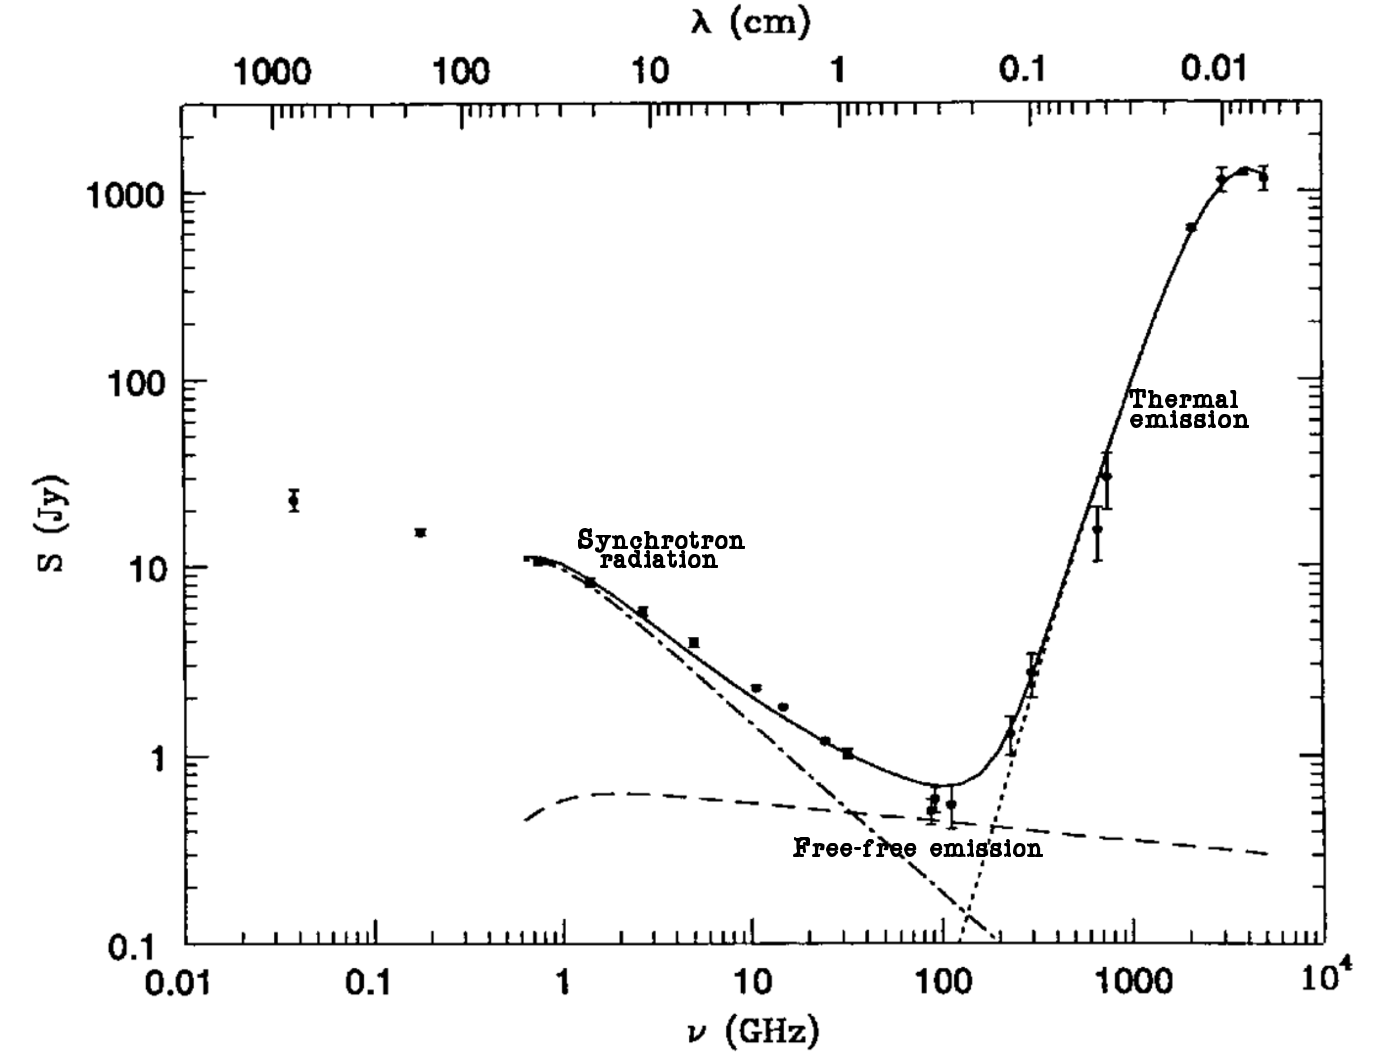
\includegraphics[scale = 0.2]{sed_edit.png}
\caption{This is the Spectral Energy Distribution of M82, a starburst galaxy. The region below the frequency of 30~GHz is from non-thermal, synchrotron emission from cosmic ray electrons. Below that frequency, free-free emission from HII regions dominates, until $\sim$200~GHz \citep{sed}.}
\label{sed}
\end{figure}

\paragraph{Epoch of Reionisation KSP:} According to the $\Lambda$CDM model, there existed a stage 400,000 years after the Big Bang, when the universe became transparent leaving only a relic radiation which we now call the Cosmic Microwave Background radiaion. This era came to be known as the ``Dark ages", and happened when the ions and electron combined. It came to an end 400 million years later, when objects such as stars and Black Holes were formed, and assembled into proto-galaxies. This era came to be known as the ``Epoch of Reionization", or ``Cosmic dawn". Several questions still need to be answered about the formation of the universe, such as what resulted in the end of the Dark Ages, and what gave rise to the EoR, and how are Black holes formed? One of the best ways to understand and answer these questions is by studying redshifted HI 21~cm emission line using LOFAR core elements.

\begin{figure}[h]
\centering
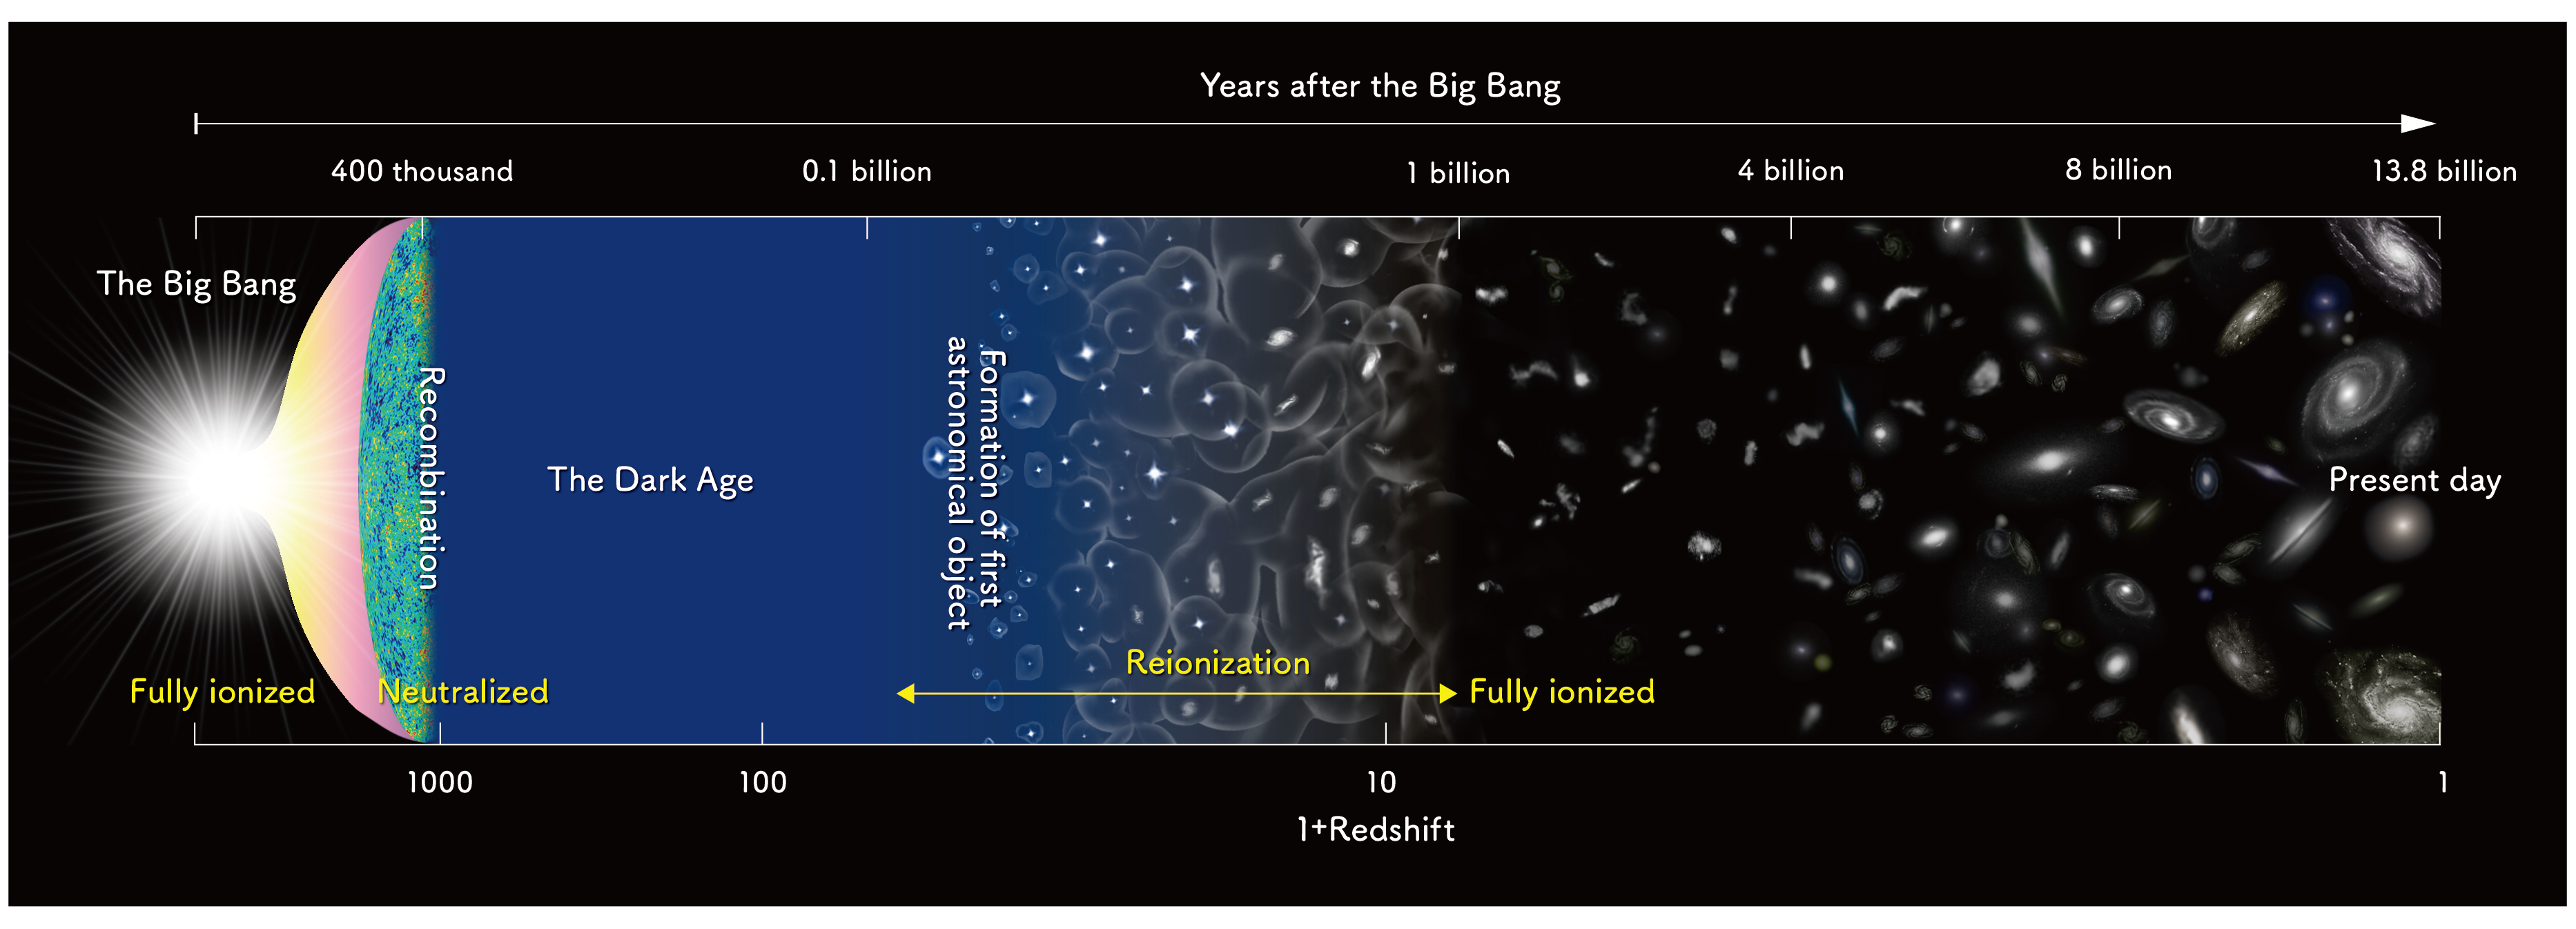
\includegraphics[scale = 0.5]{eor.jpg}
\caption{This is a schematic diagram depicting the lifetime of our universe. At redshift z$\approx$1100, the dark ages begin, and EoR begin at z$\approx$6-12. Courtesy of National Astronomical Observatory of Japan (NAOJ).}
\end{figure}

\paragraph{Surveys KSP:} LOFAR can be used for large sky surveys owing to its large instantaneous field of view. These surveys can help us study high redshifted galaxies (which will help us understand the formation and evolution of massive galaxies), clusters of galaxies (which will help us understand the charecteristics of magnetic fields and CR accelaration) and cosmic star formation history of universe.

\paragraph{Transients KSP:} This entails the study of transients such as pulsars, Gamma-Ray Bursts, X-ray binaries, radio supernovae and flare stars. Due to LOFAR's wide field and good sensitivity, it would help us do extensive time-domain studies, and discover new transient events.

\paragraph{Cosmic Rays KSP:} The Cosmic Ray (CR) flux follows the simple power law: $\frac{dN}{dE} \propto E^{-\gamma}$. Hence, for energies above 10$^{19}$eV, only one particle per century per square kilometer reaches Earth. Hence, large effective areas are required to do proper statistics. At the energy of $\sim 5 \times 10^{15}$, $\gamma$ changes from 2.7 to 3.1 in the CR spectrum, and is called the ``knee" of the spectrum. After this ``knee", the composition of the CRs is not well known. This knowledge can be obtained with the help of LOFAR, which will help us understand the accelaration and propagation mechanisms, and figure out the universal accelaration process. One of the candidates for the accelaration process is the diffusive shocks in the radio lobes of radio galaxies. Furthermore, extensive research on air showers at ground level, can help us study new particle physics.

\paragraph{Solar KSP:} Sun is an intense source of radio thermal emission, and gives rise to solar flares and Coronal Mass Ejections (CMEs) which can be studied with the help of LOFAR. Sun also has an effect on the space environments, and communication technology on earth, and hence, this project mainly aims to study the space weather and solar physics.

\paragraph{Cosmic Magnetism KSP:} Magnetic fields are very important to understand the Universe. LOFAR, due to its wide bandwidth can help us do best precision studies of Faraday rotation and weak magnetic fields. With the help of Faraday tomography/ Rotation Measure (RM) Synthesis can help us obtain polarized radio synchrotron emission. This topic will be visted again in Section \ref{rmsynthesis}.

\section{Mechanisms important at Low Frequencies}
In addition to the radiation from line emission (such as HI 21cm line), we have several other astrophysical processes that give rise to radiation. In this section, we will take a look at these processes.

\subsection{Synchrotron emission:}
\label{sec:sync}
When charged particles (mostly electrons) move around magnetic field lines at relativistic speeds, they emit photons. This emission of photons is called synchrotron emission and is non-thermal, as these relativistic electrons have a power law energy distributions:

\begin{equation}
\textrm{N(E) dE = E}^{-p} \textrm{dE}
\end{equation}

\noindent Here, N(E) dE is the number of electrons per unit volume in energy interval E and E + dE, and `\textit{p}' is the electron spectral index.

\noindent Let us consider a single electron (since synchrotron emission mostly comes from accelarating electrons), moving with velocity {\textbf{\textit{v}}} in a magnetic field {\textbf{\textit{B}}}. The electron energy is given by E = $\gamma$ mc$^2$, where $\gamma$ is the Lorentz factor and c is speed of light, and m is mass of electron. Its motion can be described by:

\begin{equation}
\frac{\textrm{d}}{\textrm{dt}} (\gamma \textrm{m}  {\textbf{\textit{v}}} ) = \frac{\textrm{e}}{\textrm{c}} (  {\textbf{\textit{v}}} \times  {\textbf{\textit{B}}} )
\end{equation}

\noindent If we resolve {\textbf{\textit{v}}} into components parallel and perpendicular to the magnetic field represented as  {\textbf{\textit{v$_{\|}$}}} and {\textbf{\textit{v$_{\bot}$}}}, then {\textbf{\textit{v$_{\|}$}}} remains constant with request to time, and $\frac{ \textrm{d{\textbf{\textit{v$_{\bot}$}}}}}{dt}$ = $\frac{\textrm{e}}{ \gamma \textrm{mc} }$ ({\textbf{\textit{v$_{\bot}$}}}$\times${\textbf{\textit{B}}})

\noindent The elctron thus moves in a helical path centered at the magnetic field lines. The pitch angle, $\theta$, of the trajectory of electron can be easily obtained from the velocity components. The angular gyrofrequency is given by the equation:

\begin{equation}
\omega_g = \frac{\textrm{e}{\textbf{\textit{B}}}}{\gamma \textrm{m}}
\end{equation}

\noindent From the figure \ref{sync}, we can see that the electron will radiate in the Lorentz transformed beam pattern, and the forward power is in the beam of the angle $\frac{2}{\gamma}$.  

\begin{figure}[h]
\centering
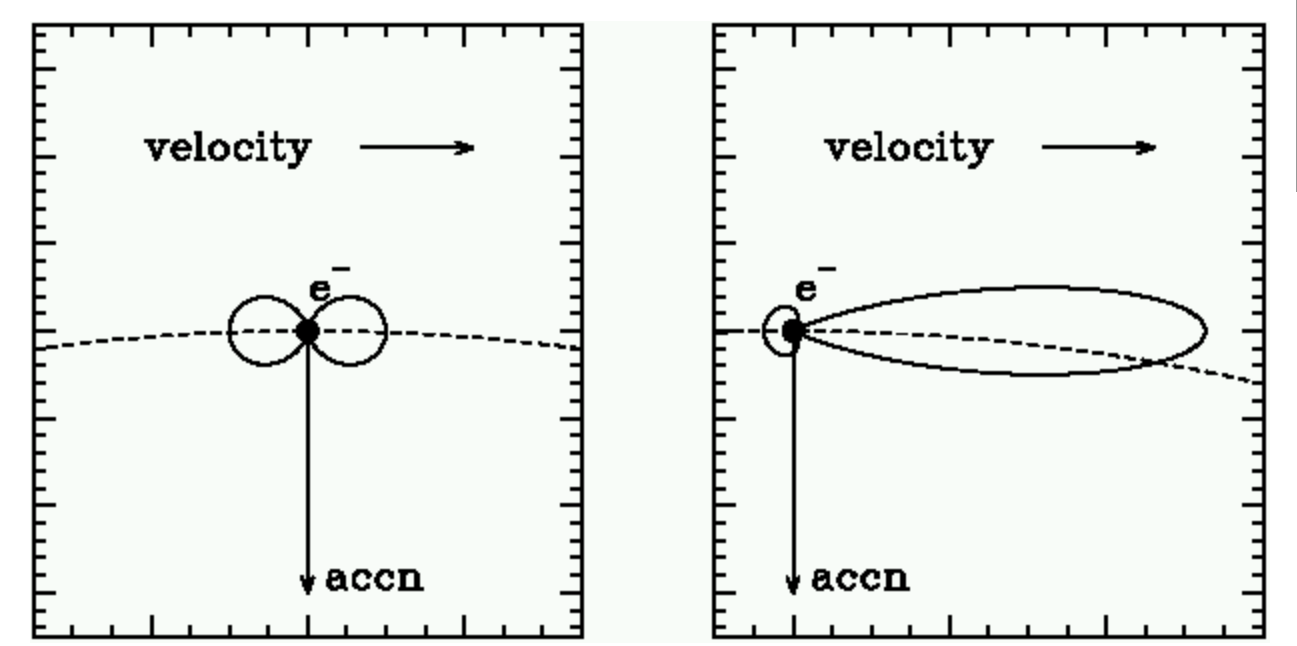
\includegraphics[scale = 0.2]{sync.png}
\caption{When an electron moves at relativistic speeds, the sin$^2$ radiation pattern is Lorentz transformed. \textit{Left:} The radiation pattern of a non-relativistic electron. \textit{Right:} The relativistic radiation pattern. This image has been taken from \url{http://www.astro.utu.fi/~cflynn/astroII/l4.html}}
\label{sync}
\end{figure}


\noindent The full derivation of the emission spectrum for a single electron can be seen in \citep{longair}. Here, I have merely written down the final equation. $I_{\|}$ and $I_{\bot}$ represent the the polarisations of the emission and $T_r$ represents the period of the electron in orbit.

\begin{equation}
j(\omega) = \frac{I_{\|} + I_{\bot}}{T_r} = \frac{\sqrt{3} e^3 \textbf{\textit{B}} sin \theta }{8 \pi^2 \epsilon_0 cm}
\end{equation}
Here, $F(x) = x \int_x ^{ \infty } K_{\frac{5}{3}} (z) dz$ where $K_{\frac{5}{3}}$  is the modified Bessel function of the order $\frac{5}{3}$ and $x= \frac{2\omega a }{3c \gamma^3}.$
From this equation, one may find the emission from a population of electrons which is seen in synchrotron emission. For the distribution of electron described earlier, the total emission for electrons with a constant pitch angle can be given by:
\begin{equation}
J(\omega) \propto \kappa \textbf{\textit{B}}^{\frac{(p+1)}{2}} \omega^{-\frac{(p-1)}{2}}
\end{equation}
Hence, the spectral index of synchrotron emission is represented as $\alpha$ and is equal to the power on the omega function.


\end{document}
